\chapter{Flat Scan Sampling}

	Background for the Flat Scan Sampling (FSS) method and a general description are presented along with the writer's C++ single core implementation details,the method's validation and proof of convergence, a short analysis of the skip parameter and a comparison with WL sampling.

\section{Background}

	The author of FSS, João Amaral, had previously, in 2014, proposed a new method to estimate the JDoS, Random Path Sampling (RPS) \cite{Amaral2014}.  The RPS was implemented in high performance languages and extensively studied by Nuno Fortunato \cite{Fortunato2015,Fortunato2016,Korotana2016}. 
	
\begin{figure}[h]
	\centering
	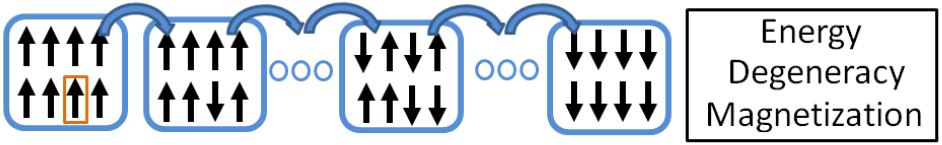
\includegraphics[scale=0.35]{rps_diagram.png}
	\caption{Scheme of how the Random Path Sampling method works.}
	\label{rps_dia}
\end{figure}
	
	The RPS method departs from the premise that by starting on an extreme magnetization point in the phase space, generally all spins up $(M)$, and successively flipping one spin down at each step of the random walk, we arrive at the other end of the phase space $(-M)$. Process illustrated in Figure \ref{rps_dia}. Performing $R$ sweeps of the phase space generate a histogram that is flat in magnetization and we can obtain the JDoS by 
\begin{align}
	H(E, M)/R &= P(E, M), \\
	\Omega(M) \times P(E, M) &= g(E, M).
\end{align}
$\Omega(M)$ is defined in Equation \ref{norm_fact}.

	The idea for FSS departs from the basic mechanism of RPS, in the sense that it is a method that estimates the JDoS by a sequential sweep of the phase space magnetization by magnetization. However the way of that both methods sample the phase space is completely different. The FSS takes a similar approach to the WL method, in the sense that a random walk with probability proportional to the inverse of the DoS is performed, a flat energy random walk.
	
	\pagebreak

\section{Algorithm}

	The Flat Scan Sampling method stems from the observation that if  the DoS at a certain magnetization $M_q$ is known, by performing a random walk the energy space $(E, M_q)$, with a probability proportional to the inverse of the DoS $\frac{1}{g(E)}$, called a flat energy random walk, and by sampling a set number of statistically diverse configurations for each energy value the DoS at the next magnetization $M_{q+1}$ can be estimated. 
This is possible because at each step of the random walk we perform a scan, i.e., in a sequential manner, we flip and unflip each spin in our configuration obtaining information about the DoS at the next magnetization, $g(E, M_{q+1})$. 
The value of $g(E_j, M_{q+1})$ is then computed through the value of $g(E_i, M_q)$ by the following equation
\begin{equation}\label{eq:FSS_JDoS}
	g(E_j, M_{q+1}) = g(E_i, M_q) \times \text{fraction of configurations}.
\end{equation}

\begin{figure}[h]
	\centering
	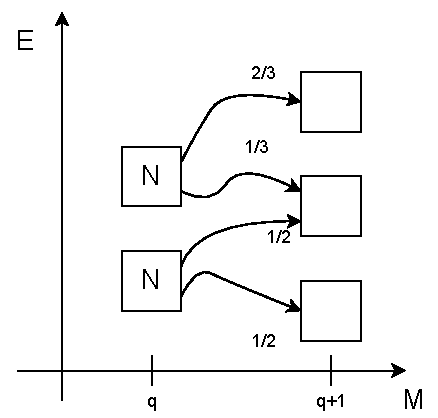
\includegraphics[scale=0.5]{fss_diagram.pdf}
	\caption{Scheme of how the Flat Scan Sampling works.}
	\label{fss_dia}
\end{figure}

Shown in Figure \ref{fss_dia}, the fraction of configurations corresponds to the fraction of the scanned configurations in the random walk that contributed to the estimation of the DoS at the next magnetization. This way, the JDoS is computed sequentially by starting at a known DoS in the phase space, such as all of the spins up $(M)$, and sweeping the whole phase space magnetization by magnetization until we arrive at the configuration where all of the spins are down $(-M)$.

The principal parameter of the method is the maximum number of samples for each point in the energy space, known as REP. In later section new parameters will be introduced to try to make the estimation more accurate while sacrificing some performance.  There will be also an extensive study of how this parameters affects the precision of the JDoS and wall time.

The algorithm can be written in the following steps:
\begin{enumerate}
\item Choose a magnetization value where $g(E, M_q)$ is known, usually magnetization where the spins all up/down;
\item Generate a certain configuration in that magnetization and compute its energy, $E_i$;                                                                                                                                       
\item Choose a spin to flip down and another one to flip up and compute the energy of the new configuration, $E_j$;
\item Accept the new configuration with a probability $\min(1, g(E_i)/g(E_j))$;
\item Sequentially flip each spin in the configuration, taking the system from the state $(E_i, M_q)$ to $(E_j, M_{q+1})$ and accumulate a histogram $H(E_i, E_j)$ and unflip the spins;
\item If the all of the number of sampled states per $(E,M_{q})$ pair is equal to REP, stop the simulation and compute the DoS at $q+1$ by using Equation \ref{eq:FSS_JDoS}. Where the fraction of configurations is now equal to $H(E_i, E_j)/\sum_j(H(E_i,E_j))$.
\end{enumerate}

\section{Implementation}

	C++ was the preferred language because of it's speed and optimization over python or Mat Lab, and modularity, over C. The random number generator (RNG) used was the xoshrio256**.

	Before the description of the implementation let us define the function that handles the scan. This should be performed each step of the simulation. The scan is defined as flipping each spin in the configuration, measuring the new energy and registering the change in state $E_i \rightarrow E_j$ in the histogram. Thus, this operation can be implemented with a for cycle running from $0$ to $N$, the number of spins.
\begin{algorithm}
	\begin{algorithmic}[1]
	\Function{\texttt{scan}}{\texttt{configuration}}	
		\For {\texttt{idx = 0,1,..., N-1}}
			\State flip the spin \texttt{idx} spin down
			\State compute the new energy \texttt{Ej}
			\State \texttt{H(Ei, Ej)++}
			\State flip the spin \texttt{idx} spin up
		\EndFor
	\EndFunction
	\end{algorithmic} 
\end{algorithm} 

	The actual implementation follows the base-line algorithm described in the last section. By knowing that the JDoS is symmetric, to save computing time, we can estimate only half of the JDoS and after the simulation mirror it. Here \texttt{qmax} is the index of the last magnetization in our computation. The variable \texttt{hist(E)} is used to count how many configurations were sampled in each point of the energy space. We only stop when every point has sampled REP microstates. In pseudo-code it can be written as follows 
	
\begin{algorithm}
	\begin{algorithmic}[1]
		\For {\texttt{q=0,1,...,qmax}}
		 	\State set \texttt{hist(E) = 0} and \texttt{H(Ei,Ej)=0}
		 	\State generate random configuration with \texttt{M=Mq} and compute its energy \texttt{Ei}
		 	\State \texttt{scan(configuration)}
		 	\State \texttt{hist(Ei)++}
		 	\While {\texttt{min(hist(E) < REP)}}
		 		\State flip one random spin down
		 		\State flip one random spin up
		 		\State compute the energy of the new configuration \texttt{Ej}
		 		\State set \texttt{ratio = min(g(Ei)/g(Ej))}
		 		\If {\texttt{rand() < ratio}}
					\State accept new configuration
				\Else
					\State reject new configuration
		 		\EndIf
		 		\If {\texttt{hist(Ei) < REP}}
		 			\State \texttt{hist(Ei)++}
			 		\State \texttt{scan(configuration)}
		 		\EndIf
		 	\EndWhile
		 	\State set \texttt{g(E,Mq+1) = g(E,Mq) * H(Ei, Ej) / sum(H(:,Ej))} 
		 \EndFor
	\end{algorithmic} 
\end{algorithm}

	This implementation has the same problem as the original WL method. We sample successive configurations, thus reducing statistical accuracy and increasing correlation between scans. This way, a new parameter that reduces correlation between scanned configurations is proposed. It is called skip and acts the same way as the parameter $S$ in the WL. We only sample configurations that are distanced by skip steps in the random walk. Only line 17 is modified by the addition of "and \texttt{k \% skip = 0}". Usually this value is set equal to the number of spins in the system, $N$, since, in theory, given $N$ steps in the random walk it might be enough to shuffle the whole configuration. As we will see in the next section, this might not be the best case, and keeping increasing this value might have diminishing returns.
	
\section{Validation and Convergence}

	We will validate FSS in two steps. The first is to show that the method is able to explore the phase space of the system correctly as it is imperative that it does. The second is to verify that the values sampled phase space give a reasonable estimate. This can be verified by computing the mean absolute error of the estimated JDoS against the exact JDoS, given by the formula
\begin{equation}\label{mean_error}
	  \langle |\epsilon|\rangle = \sum_{E, M} \frac{|g(E, M) - g_e(E, M)|}{g_e(E, M)}.
\end{equation} 
Here $g_e(E, M)$ represents the exact joint density of states.As the largest system that we have access to the exact solution is the L4 SS lattice, all of the following studies will be done for that system.

	During the flat energy random walk, there is no guarantee that the method will  be able to find all of the energies correctly. For low enough values of REP, the random walk might end before the whole energy space is discovered. When just one point in the energy space, during one iteration of the method, is not discovered, the method might not converge to a stable solution, since we use the DoS computed in the last iteration to estimate the new DoS for $M_{q+1}$. For reasonable REP values, the method does explore the whole phase space available to the system.
\begin{figure}[h]
	\centering
	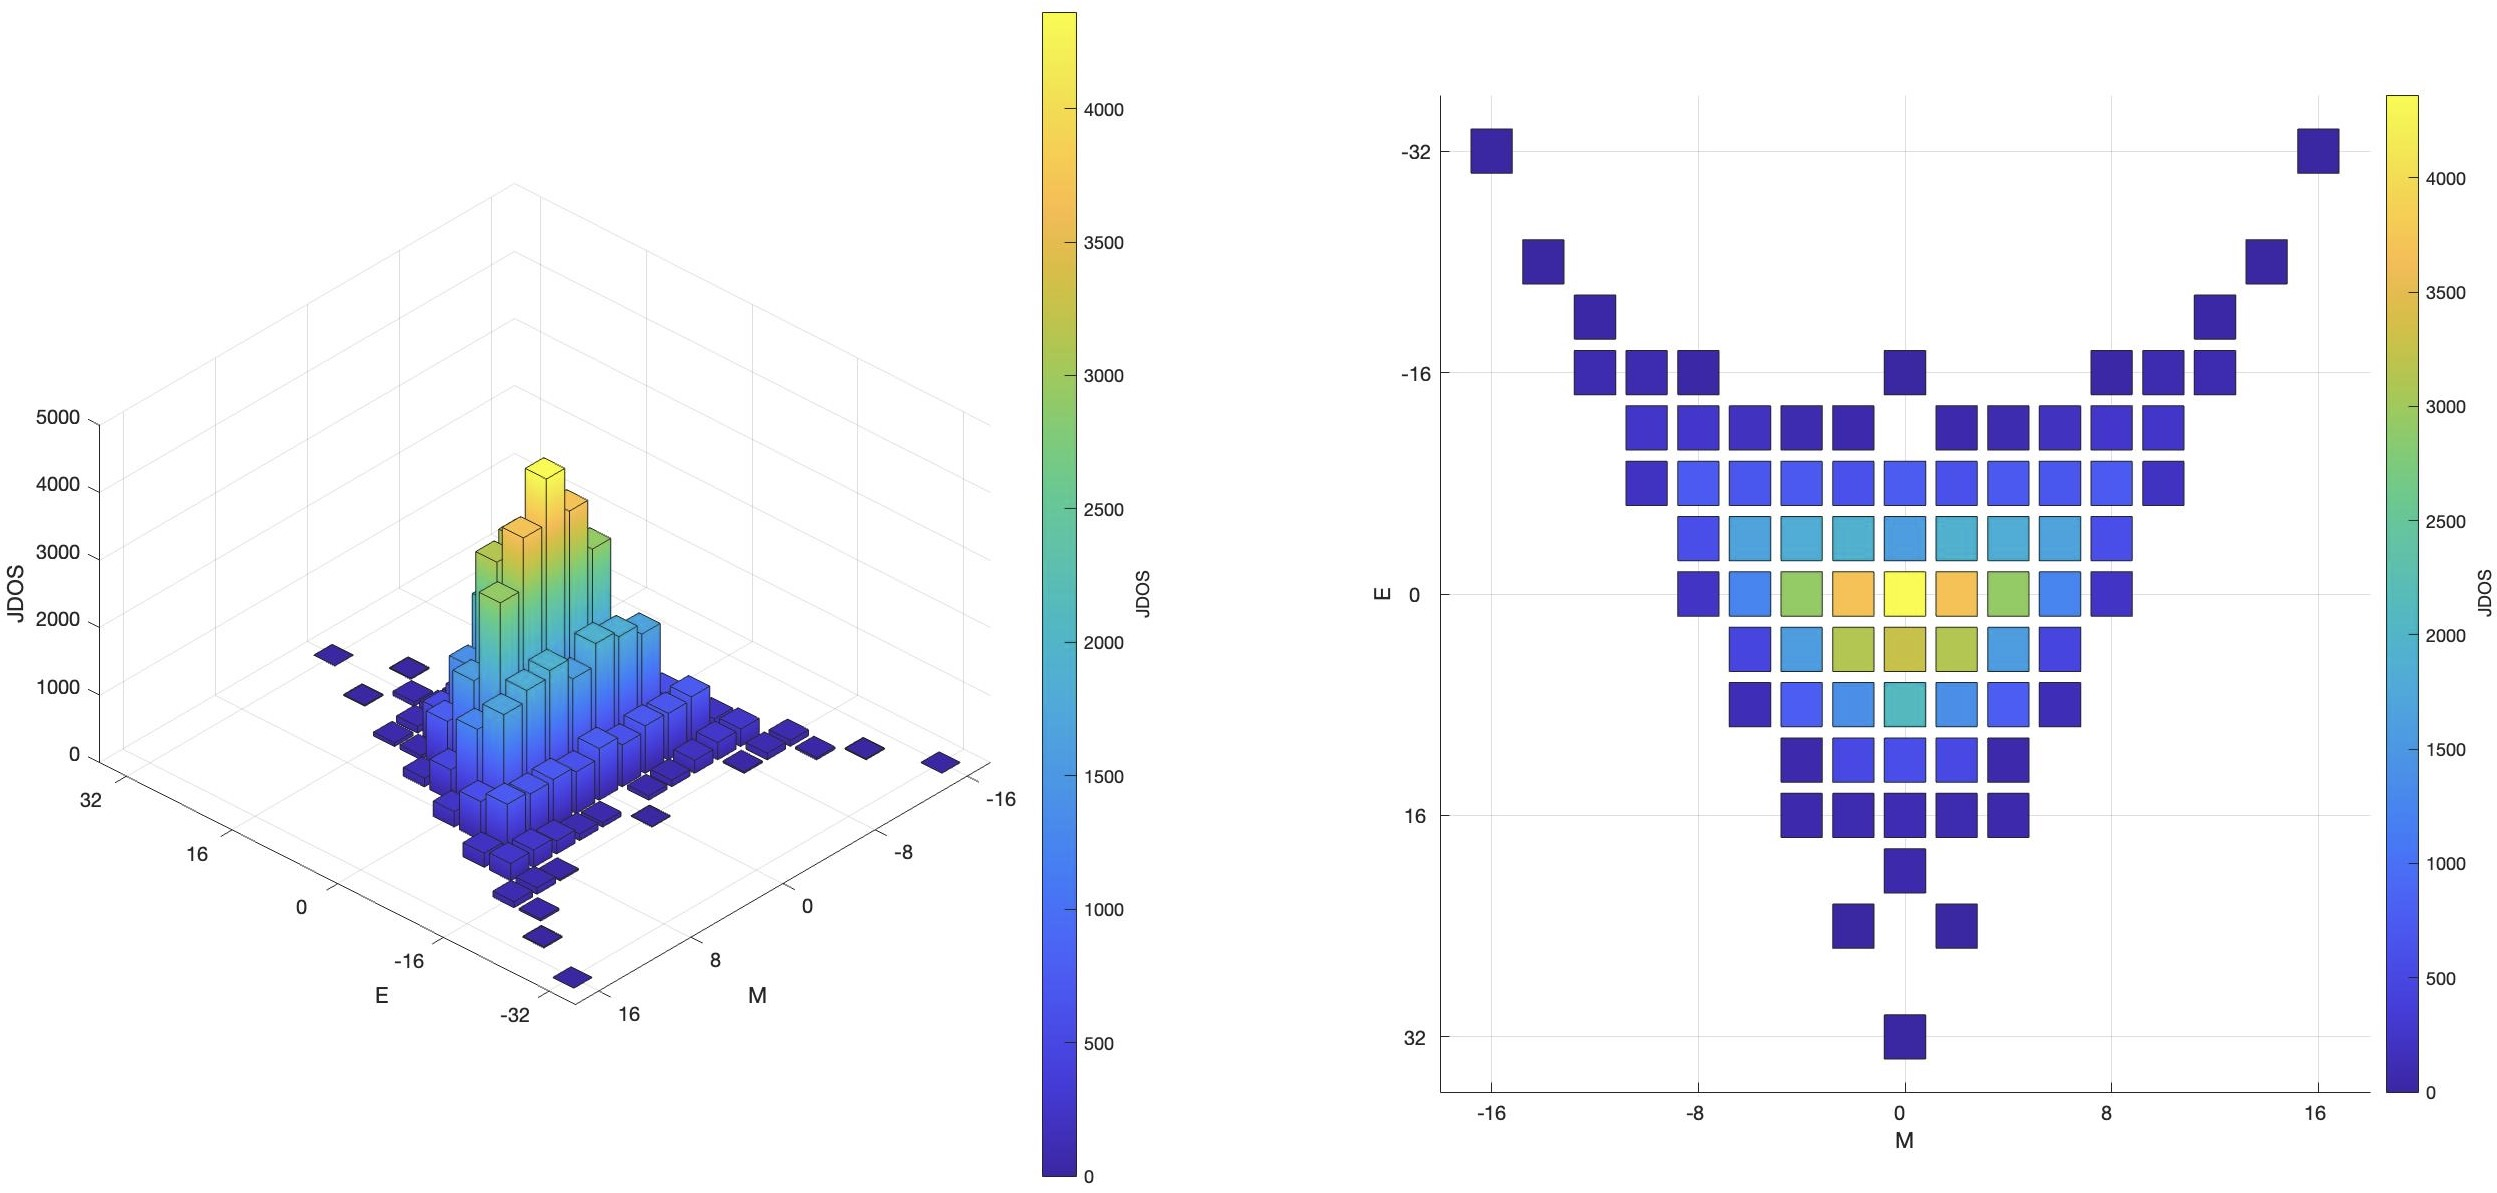
\includegraphics[scale=0.15]{convergence_validation/JDOS_L4_SS_FSS.jpg}
	\caption{Joint density of states for an L4 Ising system in a simple square lattice computed by the Flat Scan Sampling method. }
	\label{jdos_est}
\end{figure}	

\pagebreak
	
	In Figure \ref{jdos_est}, we can see the JDoS computed by the FSS method for an L4 Ising square lattice. Comparing with the phase space of the exact solution for L4 SS Ising system, Figure \ref{exact_L4}, we can see that, in fact, the whole phase space was correctly explored meaning that the FSS method is able to correctly discover all of the macrostates available to the system. 

	Since the method can find all of the points in the phase space correctly, let us now study how exact and precise those estimations are. For the second part of the validation of the method, let us study how the mean absolute error, Equation \ref{mean_error}, changes with different REP and skip values.

\begin{figure}[h]
	\centering
	\subfigure[]{
	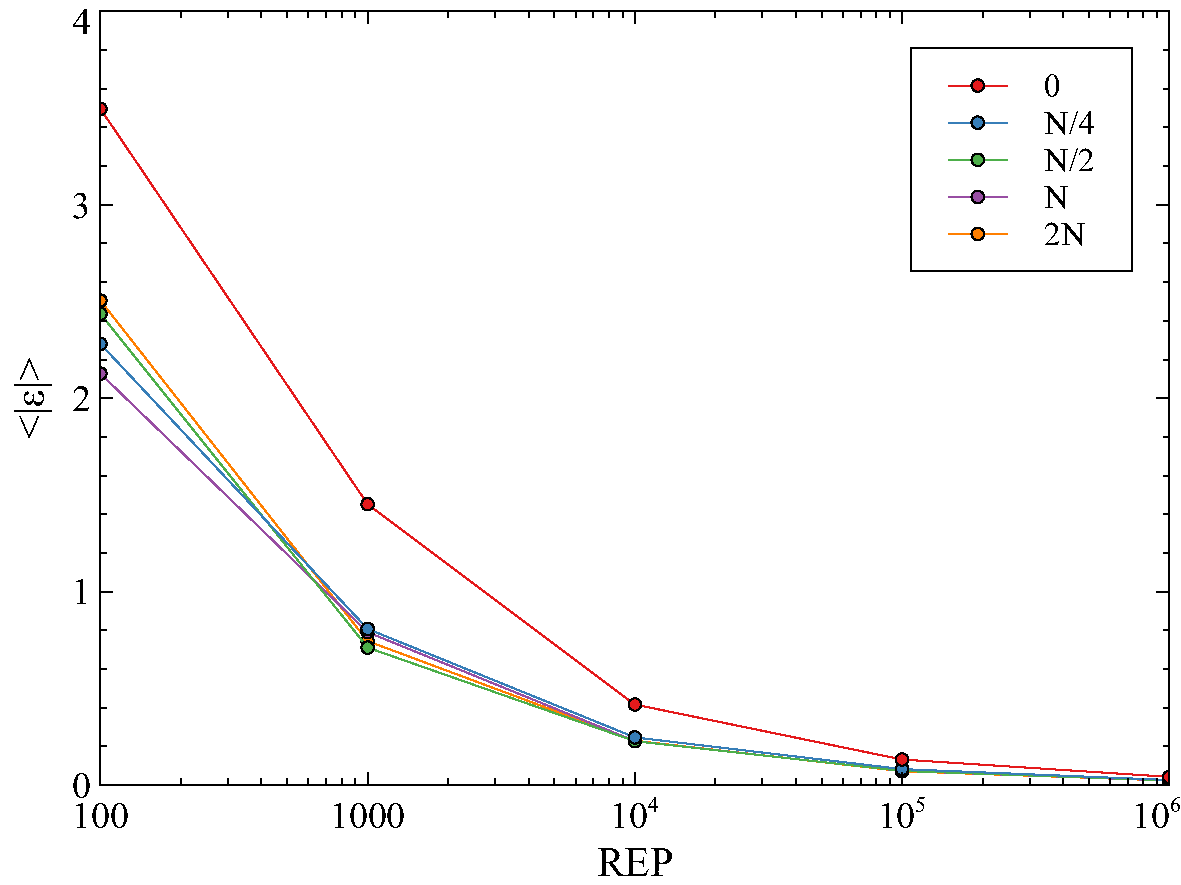
\includegraphics[scale=0.37]{convergence_validation/validation_skip_rep_01.pdf}
	\label{mean_abs_error}}
%	\quad	
	\subfigure[]{
	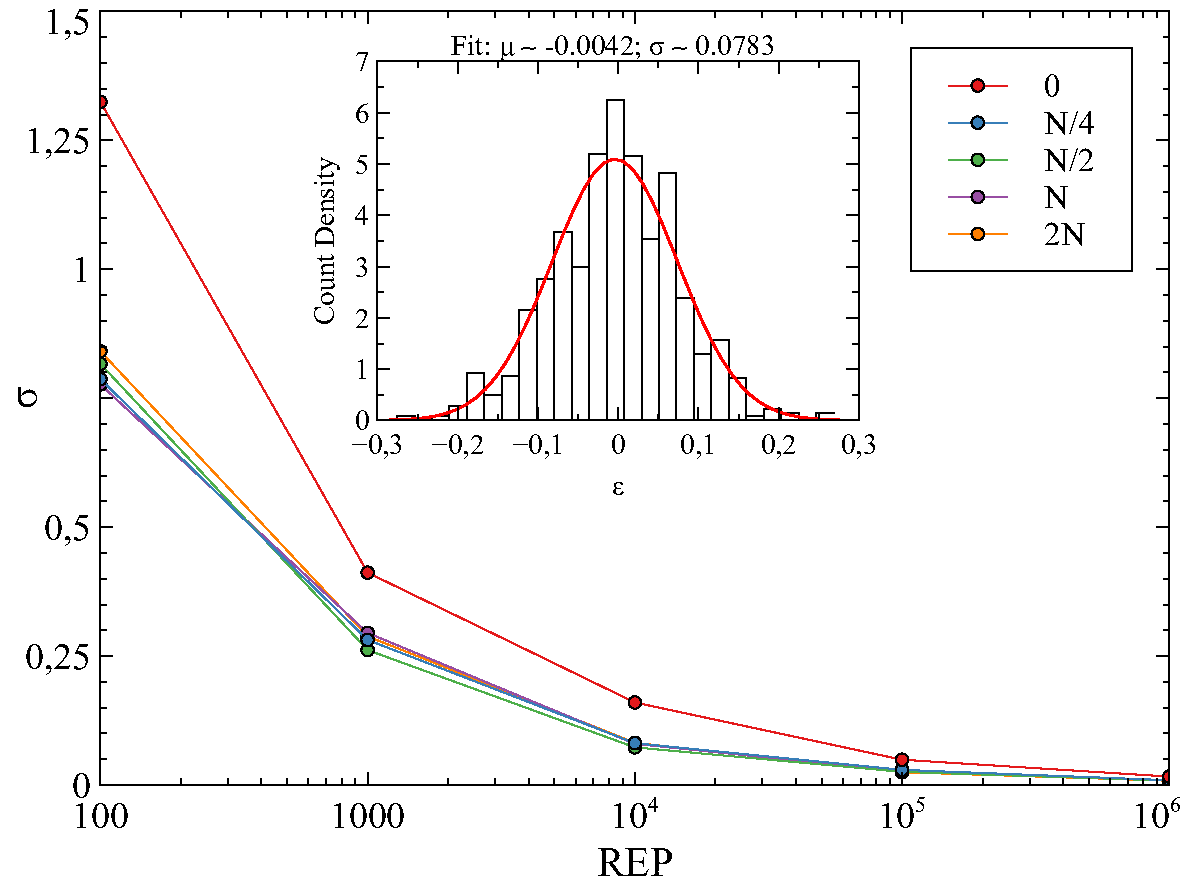
\includegraphics[scale=0.37]{convergence_validation/validation_skip_rep_02.pdf}
	\label{sgima_error}}
	\caption{(a) Mean value of the absolute error for the L4 SS JDoS, Equation \ref{mean_error}, computed by the Flat Scan Sampling method. (b) Variance of the error of the configurations as a function of REP. The inset is the fit from which the variance was taken from. Both of the plots, (a) and (b), feature various skip values, $0$, $N/4$, $N/2$, $N$ and $2N$. The results were average between 1000 simulations to reduce statistical errors.}
\end{figure}

	The mean absolute error from the JDoS for and L4 SS Ising system computed by FSS for different skip and REP values is represented in the Figure \ref{mean_abs_error}. As we increase REP, the absolute error of the JDoS converges to zero, linearly with the value of REP. Thus we can have very accurate results from the method at the cost of computing time. 
Moreover, for different values of skip, the tendency is for the error to get smaller and for small REP values, as we increase skip, the the estimated JDoS becomes more exact while for larger REP values, this increase in accuracy is not as noticeable.

	Another crucial aspect when performing a statistical analysis of a Monte Carlo is to study the convergence of the solution. We can study this by determining the mean deviation of the error. There are many ways to find the mean deviation. For this case, as the error follows a normal distribution, inset Figure \ref{sgima_error}, the mean deviation is the width of the normal distribution curve. In this case the mean deviation gives us the range of values for the error of a random FSS simulation. In Figure \ref{sgima_error}, we can see that as we increase the number of samples, the mean  deviation of the error of Flat Scan Sampling computations diminish to a value that seams close to zero.
	
	A typical behaviour of the mean deviation $\sigma$ for a Monte Carlo method is to be linearly proportional to the inverse square-root of number of samples taken to construct the solution \cite{Landau_Book}. For the FSS method, the number of steps is proportional to the value of REP, since each point in the phase space has to be sampled REP times. So, for this method the relationship should follow 
\begin{equation}\label{standard_mc}
	\sigma \propto \frac{1}{\sqrt{REP}}.
\end{equation}

	By the analysis of Figure \ref{sigma_rep}, we can see a clearly linear relationship between the mean deviation $\sigma$ and $1/\sqrt{REP}$, meaning that the convergence of FSS is linear with $1/\sqrt{REP}$. Moreover, the inset shows the extrapolation of the mean deviation for an infinite an infinite number of samples per point in the phase space. As we should expect by the analysis of Figure \ref{sgima_error} the variance vanishes as we increase REP. Therefore we can make the simulations as precise as possible at the cost of more computing time by increasing REP.
	
\begin{figure}[h]
	\centering
	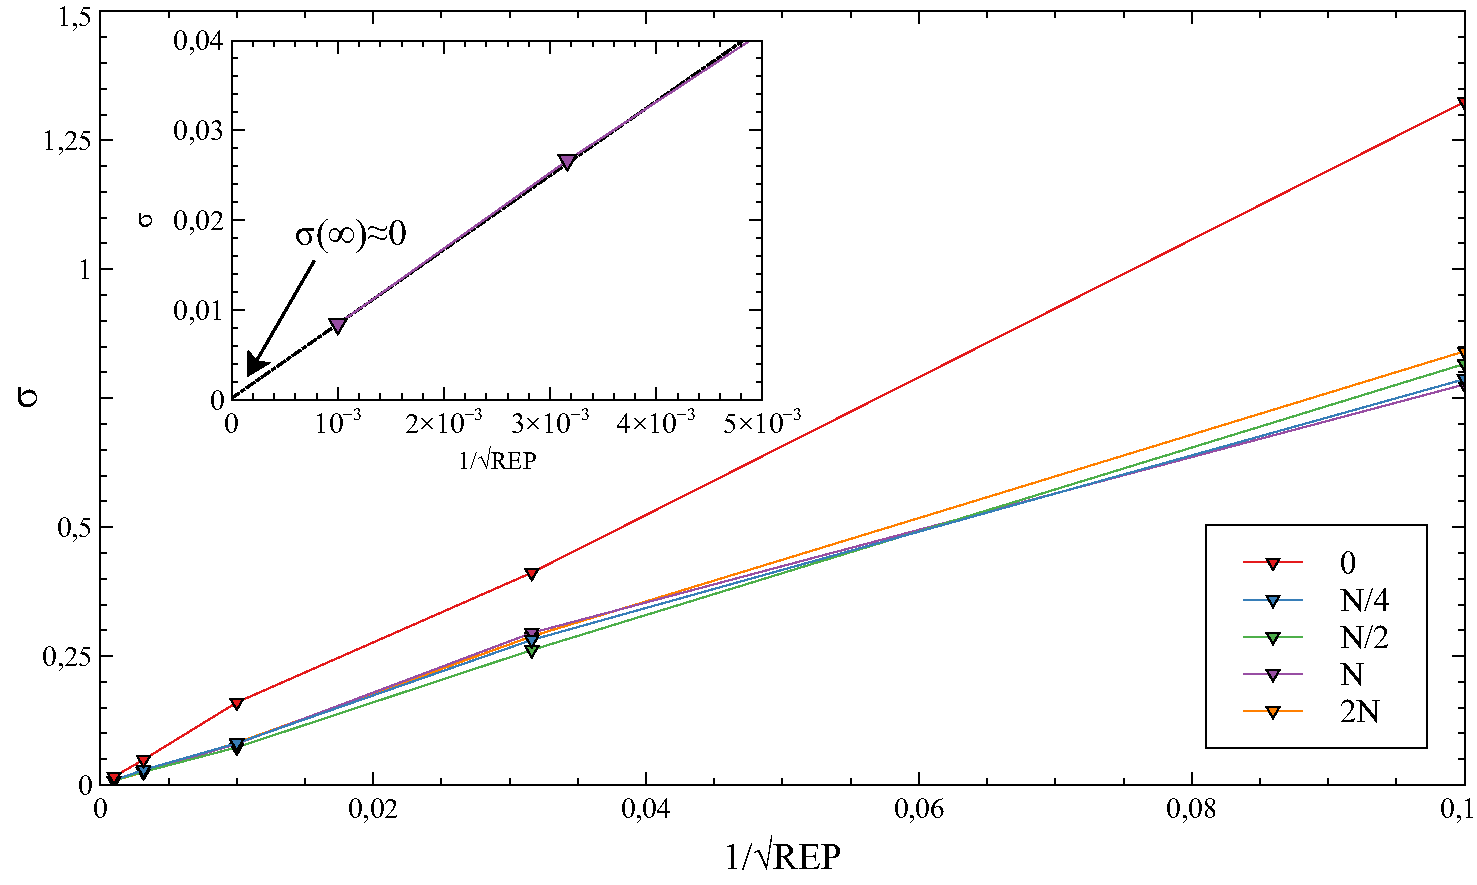
\includegraphics[scale=0.5]{convergence_validation/validation_skip_rep_03.pdf}
	\caption{Mean deviation as a function of the inverse square-root of REP.}
	\label{sigma_rep}
\end{figure}

	After this study there are three main conclusions to be taken. Flat Scan Sampling method is able to, correctly, find all of the macrostates available to a given system, the method is very accurate as we increase REP, i.e. the error in the estimated results vanishes, and that FSS converges to the exact solution with a mean deviation proportional to the inverse square-root of REP, in other words, it behaves like a standard Monte Carlo method and as we increase REP we expect the range of values for the error to vanish.
	
\subsection{Effect of Skip}

	Figure \ref{mean_abs_error} was hinting about the behaviour of the parameter skip, with the effect of skip being more noticeable for small values of REP and being phased out when REP is high. In this section a more in depth study of the skip parameter will be given.

	The function of skip is to reduce correlation between sequent samples. This naturally leads to less statistical errors when the number of samples (REP in this case) is small. However when the number of samples is high, reducing the correlation won't yield significant results. 
	Analysing Figure \ref{mean_abs_error_skip}, we can see that the mean absolute error of the JDoS computed by FSS does not vanish when skip is increased, like it does when plotted against REP. Instead it plateaus for skip$\approx N/2$ when REP is low, and it does not have a significant effect when the REP value is high. 
	When REP is low for the system, in this case $10^2$, skip does it's function and reduces correlation between successive samples therefore reducing the mean absolute error. However, when we increase REP thus taking much more samples per point in the phase space, the correlation between them does not have much effect on the accuracy of the computation. 
	
	\pagebreak

\begin{figure}[h]
	\centering
	\subfigure[]{
	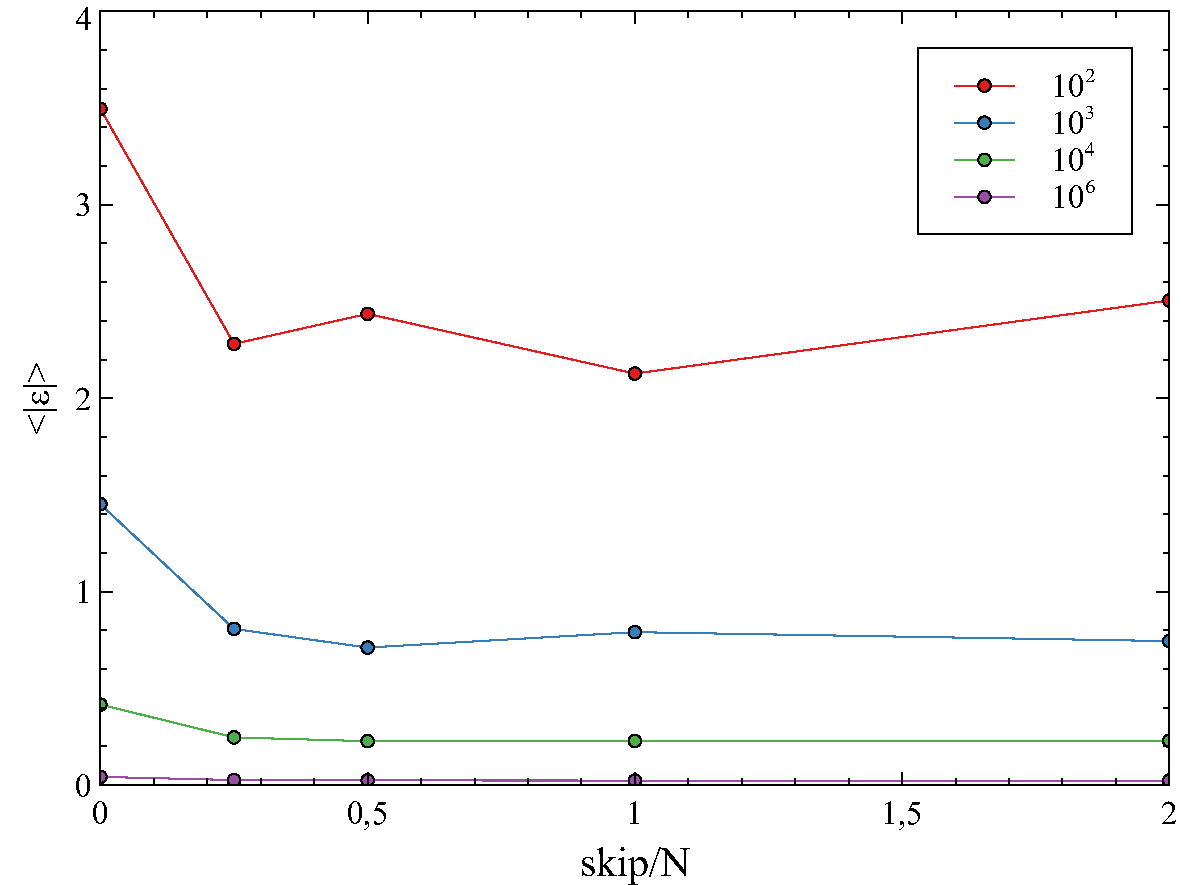
\includegraphics[scale=0.37]{convergence_validation/validation_rep_skip_01.pdf}
	\label{mean_abs_error_skip}}
%	\quad	
	\subfigure[]{
	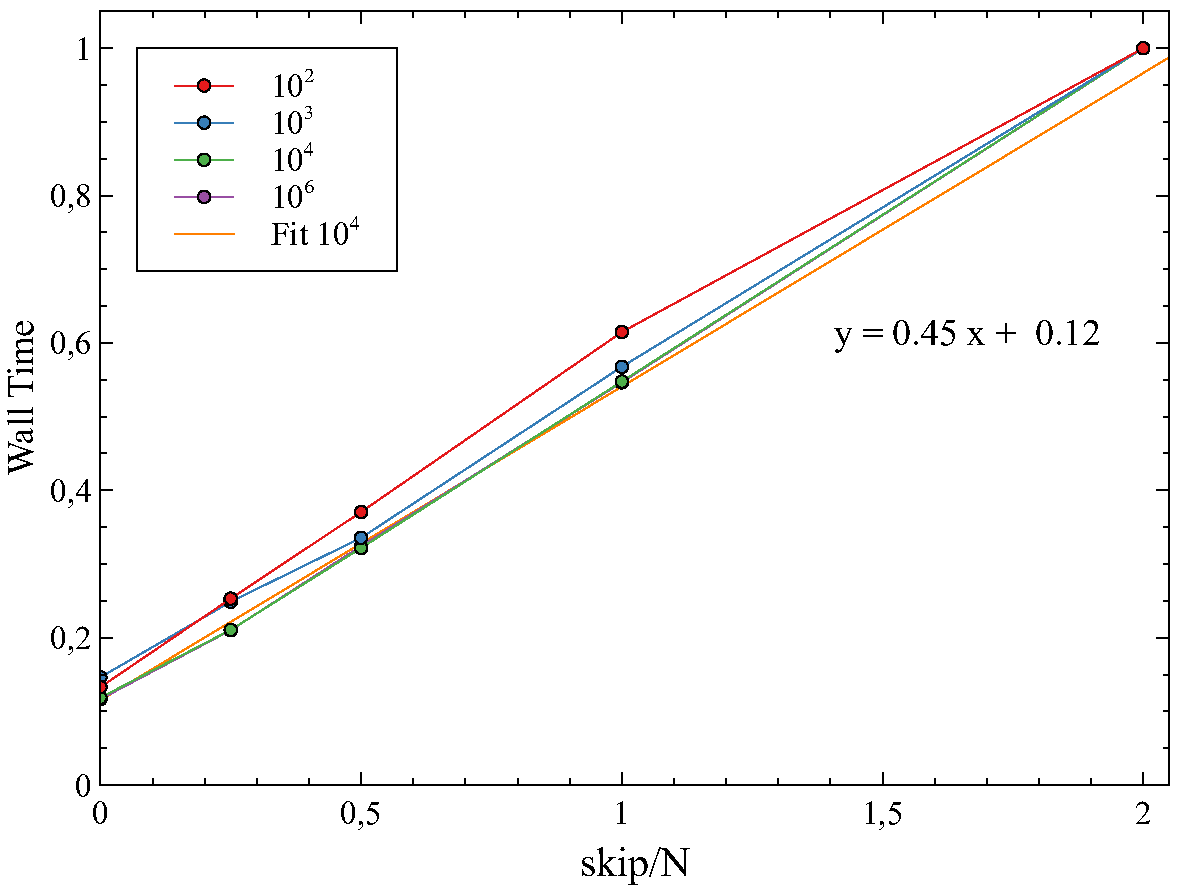
\includegraphics[scale=0.37]{convergence_validation/validation_rep_skip_02.pdf}
	\label{wall_time_skip}}
	\caption{(a) Mean absolute error of the L4 SS Ising JDoS computed by FSS method as a function of the skip parameter for various REP values. (b) Normalized wall time as a function of the skip parameter with a linear fit for the wall time of REP $=\ 10^4$. The results were averaged over 1000 simulations in order to reduce statistical errors.}
\end{figure}

	In the next section a more in depth look at the performance of FSS will be given, but it is worth noting that the wall time is linear with the skip value, Figure \ref{wall_time_skip}. The linear relation can be approximated by $y=0.45x + 0.12$. 
	
	With the insertion of the parameter skip in the FSS implementation, we can have less statistical errors while not increasing the wall time by a big margin. For skip$> N/2$ we will have diminishing returns, so the most advantageous value for skip is $N/2$ or at most $N/4$. 

\section{Comparison with Wang-Landau - Accuracy}

	Having validated Flat Scan Sampling, study it's convergence and skip parameter, let us now compare FSS to the widely accepted and studied Wang-Landau Sampling. In this section we will only compare accuracy and precision in the computations and in the next chapter after analysing the performance of FSS we will compare it to WL's performance. 
	We will be comparing results from simulations of the Ising model on a L8 simple square lattice. As we do not have the exact solutions for this lattice size, we will resort to study the two known points in the phase space, the Checker Board and the Slice. 
	
	Knowing that the Checker Board has exactly 2 configurations and that the Slice has $16\ (2 \times 8)$ configurations we can compare the precision and accuracy of both methods. In Figures \ref{ep_ch} and \ref{ep_sl} we can see the medium value of the absolute error for the two configurations. The error of the Wang-Landau computations never vanishes, therefore it converges to the wrong solution, while with Flat Scan Sampling we can get a really accurate estimation of the JDoS. 
	
	Another important aspect worth noting is the difference between the FSS precision in the Checker Board and Slice configurations. The WL computations have roughly the same error in the two configurations, instead the FSS method is less accurate in the Slice configuration. This is due to the nature of the method. As FSS estimates the JDoS in a sequential manner, and the computed JDoS is used to estimate the new one, errors are more susceptible to propagate through each iteration.
	
	\pagebreak
	
\begin{figure}[h]
	\centering
	\subfigure[]{
	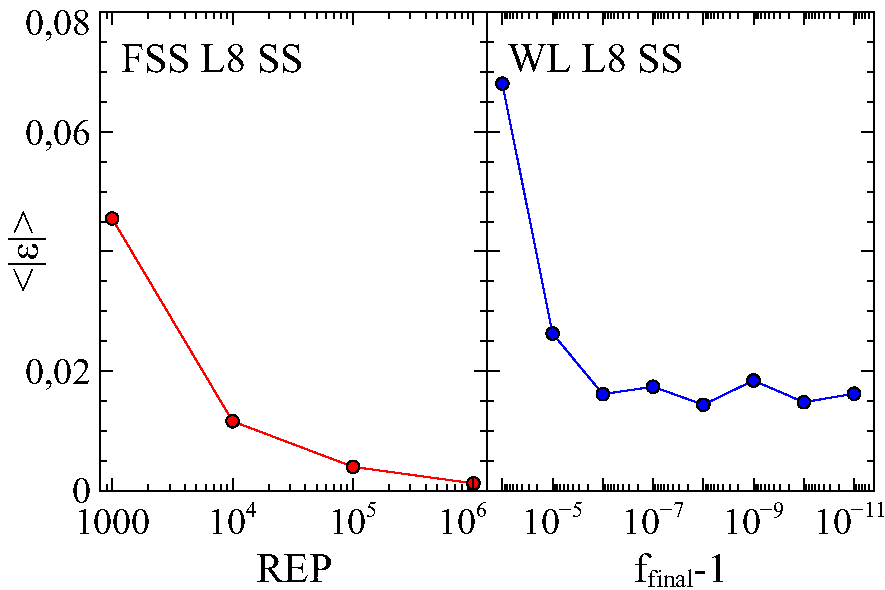
\includegraphics[scale=0.37]{comparison/wl_comp_07.pdf}
	\label{ep_ch}
	}
	\subfigure[]{
	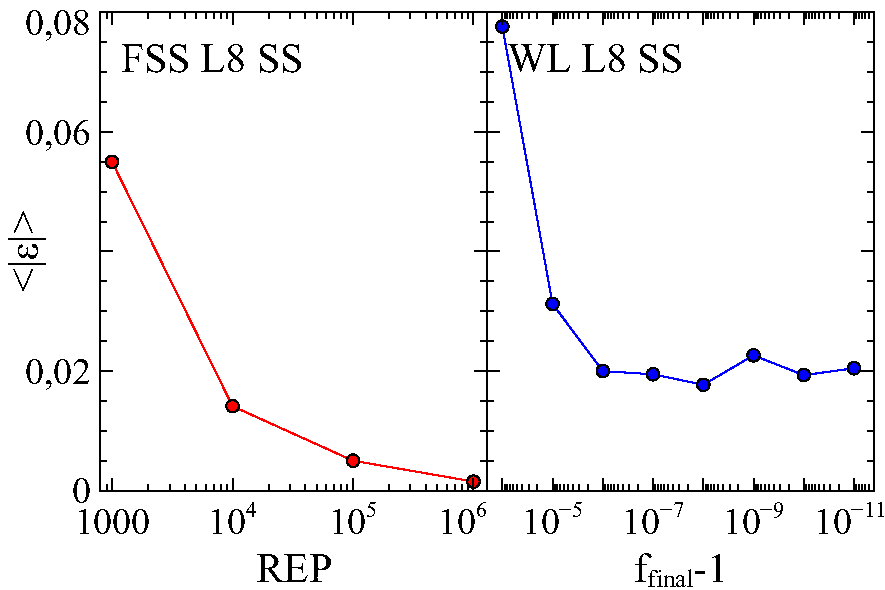
\includegraphics[scale=0.37]{comparison/wl_comp_08.pdf}
	\label{ep_sl}
	}

	\subfigure[]{
	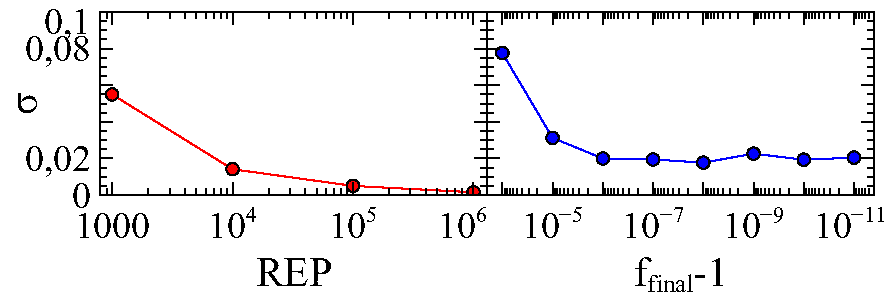
\includegraphics[scale=0.37]{comparison/wl_comp_09.pdf}
	\label{sg_ch}
	}
	\subfigure[]{
	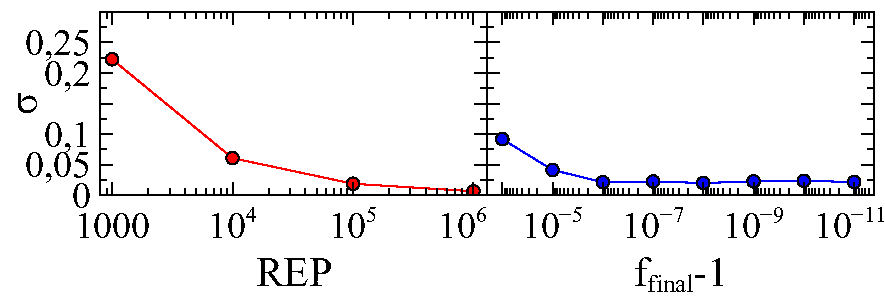
\includegraphics[scale=0.37]{comparison/wl_comp_10.pdf}
	\label{sg_sl}
	}
	
	\caption{Mean absolute error and standard deviation as a function of the method parameter for the Checker Board configuration (a) and (c) and for the Slice configuration (b) and (d). Red lines represent the results for the Flat Scan Sampling and blue lines for the Wang-Landau sampling. Results were averaged through 1000 simulations to reduce statistical error.}
\end{figure}

	As shown in the previous section the error follows a normal distribution so we can analyse it's mean deviation. In Figures \ref{sg_ch} and \ref{sg_sl} we can see the sigma values of both methods for the Checker Board and Slice configurations, respectively.For the WL sampling, the mean deviation follows the same pattern as the mean absolute error, it never vanishes, instead it converges to a non-zero small positive value. This is illustrated in Figure \ref{fit_comp}, as we can clearly see, from an extrapolation, that the mean deviation of FSS at infinite samples is zero and, at infinite steps in the random walk, the sigma for WL does not vanish but converges to a small enough value that can be ignored.

	In Figure \ref{fit_comp} we can observe that the mean deviation Flat Scan Sampling results goes to zero while being linear with REP and the WL's does not. This indicates that WL does not behave like a standard Monte-Carlo method, Equation \ref{standard_mc}. 

\begin{figure}[h]
	\centering
	\subfigure[]{
	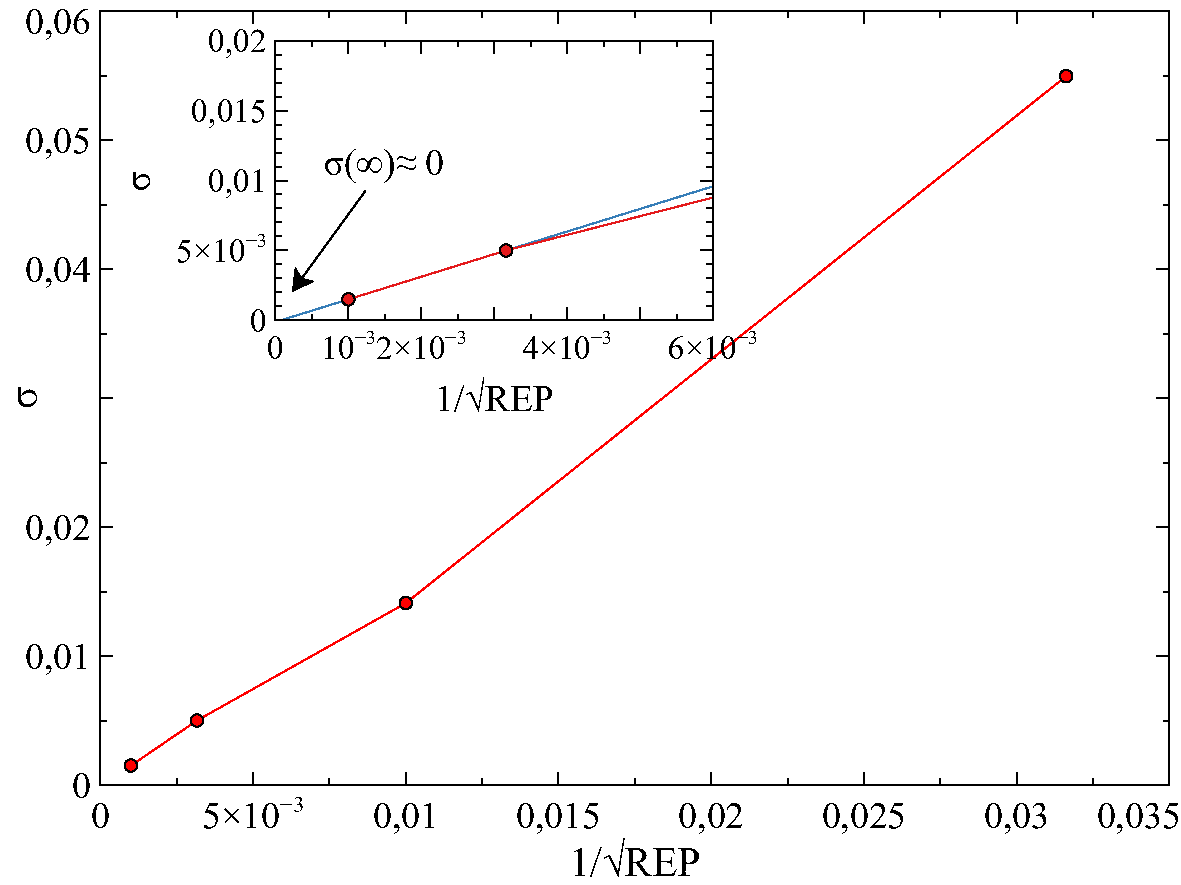
\includegraphics[scale=0.29]{comparison/wl_comp_03.pdf}
	}
	\subfigure[]{
	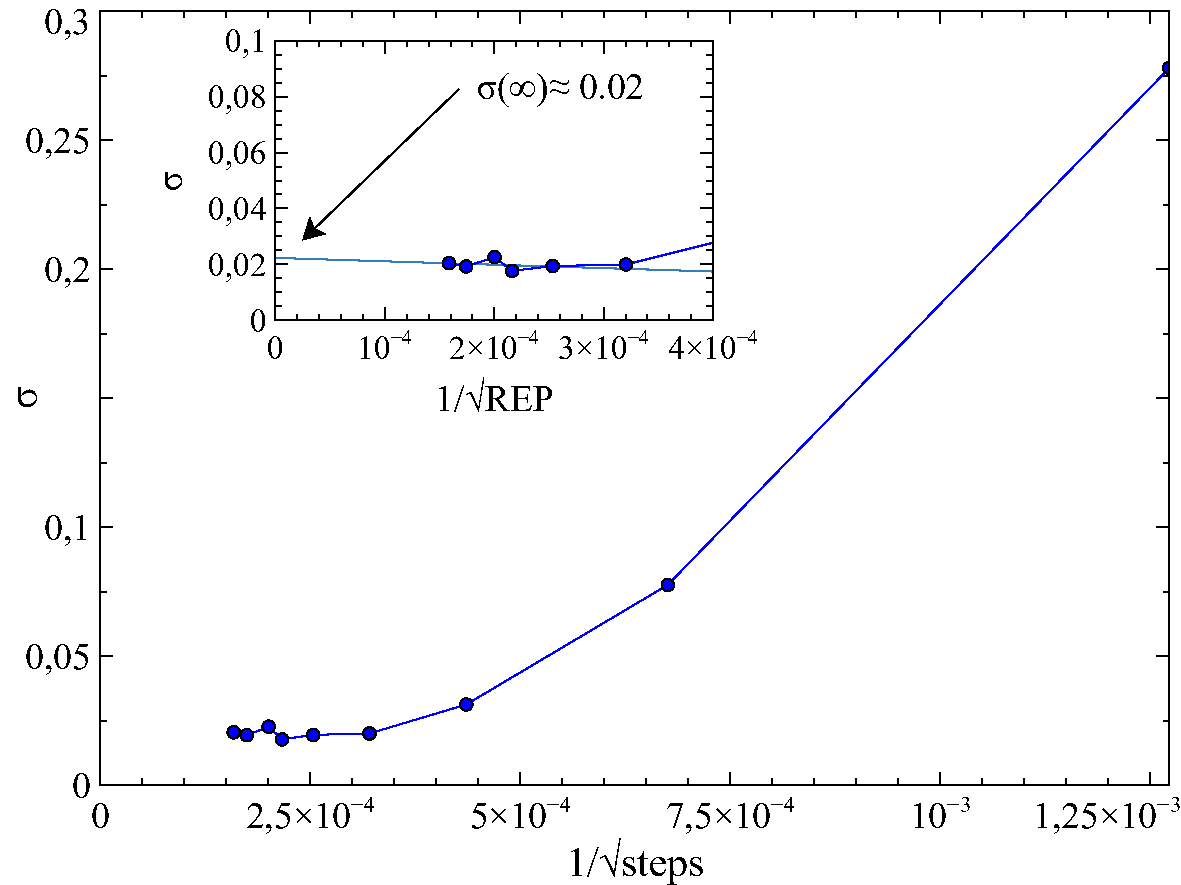
\includegraphics[scale=0.29]{comparison/wl_comp_04.pdf}
	}
	
	\caption{Mean deviation as a function of the inverse square-root of the number of steps taken in the random walk during the simulation. (a) FSS (b) WL}
	\label{fit_comp}
\end{figure}

	In Figure \ref{fit_comp} we can also see that the mean deviation Flat Scan Sampling results converges to zero while being linear with REP and the WL's does not. This shows that WL does not behave like a standard Monte-Carlo method, Equation \ref{standard_mc}.




















